% Created 2017-03-06 Mon 15:48
% Intended LaTeX compiler: pdflatex
\documentclass[a4paper,11pt]{article}
\usepackage[utf8]{inputenc}
\usepackage[T1]{fontenc}
\usepackage{graphicx}
\usepackage{grffile}
\usepackage{longtable}
\usepackage{wrapfig}
\usepackage{rotating}
\usepackage[normalem]{ulem}
\usepackage{amsmath}
\usepackage{textcomp}
\usepackage{amssymb}
\usepackage{capt-of}
\usepackage{hyperref}
\usepackage[margin=1.2in]{geometry}
\usepackage{setspace}
\onehalfspacing
\usepackage{parskip}
\usepackage{amsthm}
\usepackage{amsmath}
\usepackage{mathtools}
\usepackage{hyperref}
\usepackage{graphicx}
\usepackage{tabularx}
\usepackage{booktabs}
\hypersetup{colorlinks,citecolor=black,filecolor=black,linkcolor=black,urlcolor=black}
\newtheorem{mydef}{Definition}
\newtheorem{mythm}{Theorem}
\newcommand{\dx}{\mathrm{d}}
\newcommand{\var}{\mathrm{Var}}
\newcommand{\cov}{\mathrm{Cov}}
\newcommand{\corr}{\mathrm{Corr}}
\newcommand{\pr}{\mathrm{Pr}}
\newcommand{\rarrowd}[1]{\xrightarrow{\text{ \textit #1 }}}
\renewcommand\chaptername{Lecture}
\DeclareMathOperator*{\plim}{plim}
\newcommand{\plimn}{\plim_{n \rightarrow \infty}}
\setcounter{secnumdepth}{2}
\author{Zheng Tian}
\date{March 28, 2016}
\title{Lecture 5: Linear Regression with One Regressor}
\hypersetup{
 pdfauthor={Zheng Tian},
 pdftitle={Lecture 5: Linear Regression with One Regressor},
 pdfkeywords={},
 pdfsubject={},
 pdfcreator={Emacs 25.1.1 (Org mode 9.0.3)}, 
 pdflang={English}}
\begin{document}

\maketitle

\section{Introduction}
\label{sec:org91069ec}
This chapter introduces the linear regression model relating one
variable, \(X\), to another, \(Y\), which is called the linear regression
model with one regressor or the simple linear regression model. This
chapter describes the ordinary least squares (OLS) methods for
estimating a simple linear regression model, discusses the algebraic
and statistical properties of the OLS estimator, introduces two
measures of fit, and lays out three least squares assumptions for the
linear regression model. We apply the OLS estimation method to a
linear model of test scores and class sizes in California school
districts. 

This chapter lays out foundations for all chapters that
follow. Although in practice we seldom use a linear regression model
with only one regressor, the essential principles of the OLS estimation
method are the same for a linear regression model with multiple
regressors. 


\section{The Linear Regression Model}
\label{sec:orgb1ff2b1}
\subsection{What is regression?}
\label{sec:org4c3f4b2}
\subsubsection*{Definition of \emph{regress} in Merriam-Webster's dictionary}
\label{sec:org4dacdb1}

\begin{description}
\item[{1}] an act or the privilege of going or coming back
\item[{2}] movement backward to a previous and especially worse or more primitive state or condition
\item[{3}] the act of reasoning backward
\end{description}

\subsubsection*{The meaning of regression in statistics?}
\label{sec:org3c65071}
In statistical modeling, regression analysis is a statistical process
for estimating the relationships among variables.\footnote{Read
the article in Wikipedia
\url{https://en.wikipedia.org/wiki/Regression\_analysis}} Specifically, most
regression analysis focus on the conditional mean of the dependent
variable given the independent variables, which is a function of
\(x\). A very simple but common form of the function is a linear
function, i.e., \(\beta_0 + \beta_1 x\), such as
\begin{equation*}
E(Y | X = x) = f(x) = \beta_{0} + \beta_1 x
\end{equation*}

\subsection{An example: Test scores versus class size}
\label{sec:orgfa5ec3b}
\subsubsection*{The background of the story}
\label{sec:orgbc8de49}
The superintendent of an elementary school district is facing a
trade-off: 
\begin{itemize}
\item Hiring more teachers to improve students' test performance
\item Keeping the budget tight
\end{itemize}

\subsubsection*{Research question:}
\label{sec:org6b061ef}
Can reducing class size increase students' test scores?
\subsubsection*{How can we answer the question?}
\label{sec:orgc0b53f9}
\begin{itemize}
\item We randomly choose 42 students and divide them into two classes,
with one having 20 students and another having 22. And they are
taught with the same subject and by the same teachers.
\item Randomization ensures that it is only the difference in class
sizes of the two classes that will affect test scores.
\item After a test for both classes, we then compute the average test
scores which can be expressed as, 
\begin{gather*}
E(TestScore | ClassSize = 20) \\
E(TestScore | ClassSize = 22) 
\end{gather*}
\item Then the effect of class size on test scores can be reflected as
\begin{equation*}
E(TestScore | ClassSize = 20) - E(TestScore | ClassSize = 22)
\end{equation*}
\item If the difference is large enough, we can say that reducing class
can improve students' test performance.
\item Question: how can we relate test scores to class sizes?  The key is
in \(E(TestScore | ClassSize)\), which dictates a regression function.
\end{itemize}

\subsubsection*{A general model of test scores v.s. class size}
\label{sec:org7de9008}
Generally, we can write the \textbf{population regression line} as
\begin{equation}
\label{eq:popreg-testscore}
E(TestScore | ClassSzie) = \beta_0 + \beta_1 ClassSize
\end{equation}

By calculating the conditional expectation, some other factors apart
from class sizes may be canceled out. These factors may also influence
test scores, but they are either unimportant in your reasoning or
unable to be measured. We can lump all these factors into a
single term, and set up a general regression model as

\begin{equation}
\label{eq:regmodel-testscore}
TestScore = \beta_0 + \beta_1 ClassSize + OtherFactors
\end{equation}

If we assume \(E(OtherFactors | ClassSize) = 0\), then the linear
regression model (Eq. \ref{eq:regmodel-testscore}) becomes the population
regression line (Eq. \ref{eq:popreg-testscore}).

\subsubsection*{Explore the data with a scatterplot}
\label{sec:org64b3076}

The relationship between the data points, the population regression
line, and the errors (other factors) are illustrated in Figure \ref{fig:org3619567}.

\begin{figure}[htbp]
\centering
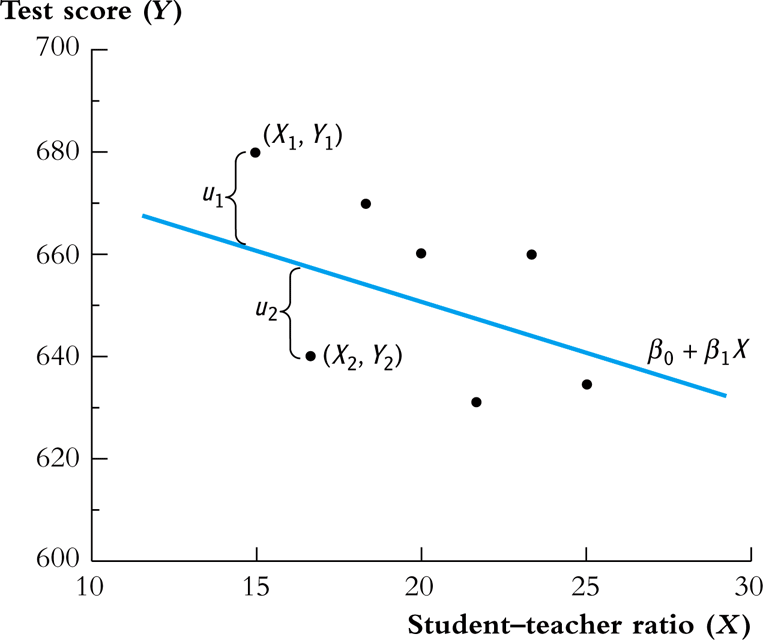
\includegraphics[width=0.75\textwidth]{img/fig-4-1.png}
\caption{\label{fig:org3619567}
The Population Regression Line}
\end{figure}

\subsection{The general linear regression model}
\label{sec:orgf451fff}

Consider two variables \(Y\) and \(X\). For both, there are \(n\)
observations so that each observation \(i (=1, 2, 3, \ldots)\) is
associated with a pair of values of \(Y_i\) and \(X_i\). What we are
interested in is how a unit change in \(X\) will affect \(Y\). For that,
we can set up a linear regression model as

\begin{equation}
\label{eq:single-regress}
Y_i = \beta_0 + \beta_1 X_i + u_i, \text{ for } i = 1, \ldots, n
\end{equation}

\begin{itemize}
\item \(Y_i\) : the dependent variable, the regressand, or the LHS
(left-hand side) variable.
\item \(X_i\) : the independent variable, the regressor, or the RHS
(right-hand side) variable.
\item \(\beta_{0}\) : the intercept, or the constant term. It can either have
economic meaning or have merely mathematical sense, which determines
the level of the regression line, that is, the point of intersection
with the Y axis.
\item \(\beta_{1}\) : is the slope of the population regression
line. \(\beta_1 = \dx Y_i/\dx X_i\) is the marginal effect of \(X\) on
\(Y\), that is, one unit change in \(X\) changes \(Y\) by \(\beta_{\text{1}}\) units,
holding other things constant.
\item \(u_i\) : is the error term. \(u_i = Y_i - (\beta_0 + \beta_1 X_i)\)
incorporates all the other factors besides \(X\) that determine the
value of \(Y\).
\item \(\beta_{0} + \beta_{1}X_{i}\) : the population regression
function/line. We can predict the value of \(Y\) given a value of \(X\)
according to the population regression line.
\end{itemize}



\section{The OLS Estimation Method for a Linear Regression Model}
\label{sec:org68288b2}
\subsection{The intuition for the OLS and minimization}
\label{sec:org2a189cc}
The most common method to estimate a linear regression model, like
Equation \ref{eq:single-regress}, is to use the ordinary least squares (OLS)
estimator.\footnote{Recall that an \textbf{estimator} is a function of a sample of
data. An \textbf{estimate} is the numerical value of the estimator when it is
computed using data from a sample.}

Let's explain the basic idea of the OLS by dissecting its name.
\begin{description}
\item[{Ordinary}] It means that the OLS estimator is a very basic method,
from which we may derive some variations of the OLS
estimator, such as the weighted least squares (WLS), and the
generalized least squares (GLS).
\item[{Least}] It means that the OLS estimator tries to minimize
something. The "something" is the mistakes we
make when we try to guess (estimate) the values of the
parameters in the model. From Equation
\ref{eq:single-regress}, if our guess for \(\beta_0\) and
\(\beta_1\) is \(b_0\) and \(b_1\), then the mistake of our guess
is \(\hat{u}_{i} = Y_{i} - b_0 - b_1 X_i\).
\item[{Squares}] It represent the actual thing (a quantity) that we
minimize. The OLS does not attempt to minimize each
\(\hat{u}_{i}\) but to minimize the sum of the squared
mistakes, \(\sum_{i=1}^n \hat{u}_i^2\). Taking square is to
avoid possible offsetting between positive and negative values of
\(\hat{u}_i\) in \(\sum_i \hat{u}_i\).
\end{description}

\subsection{The OLS estimators for \(\beta_0\) and \(\beta_1\)}
\label{sec:org35380d5}

Let \(b_0\) and \(b_1\) be some estimators of \(\beta_0\) and \(\beta_1\),
respectively. Then, the OLS estimator is the
solution to the following minimization problem.

\begin{equation}
\operatorname*{min}_{b_0, b_1}\: S(b_0, b_1) = \sum_{i=1}^n \hat{u}_i^2 = \sum_{i=1}^n (Y_i - b_0 - b_1 X_i)^2 \label{eq:min-ols}
\end{equation}

where \(S(b_0, b_1)\) is a function of \(b_0\) and \(b_1\), measuring the
sum of the squared prediction mistakes over all \(n\) observation.

\begin{proof}
We solve the problem by taking the derivative of $S(b_0, b_1)$ with respect to $b_0$ and $b_1$,
respectively. Then the first order conditions evaluated at the value of a solution $\hat{\beta}_0$
and $\hat{\beta}_1$ are

\begin{align}
& \frac{\partial S}{\partial b_0}(\hat{\beta}_0, \hat{\beta}_1) = \sum_{i=1}^n (-2)(Y_i - \hat{\beta}_0 - \hat{\beta}_1 X_i) = 0  \label{eq:b-0} \\
& \frac{\partial S}{\partial b_1}(\hat{\beta}_0, \hat{\beta}_1) = \sum_{i=1}^n (-2)(Y_i - \hat{\beta}_0 - \hat{\beta}_1 X_i) X_i = 0 \label{eq:b-1}
\end{align}

Rearranging Equation \ref{eq:b-0}, we get
\begin{gather}
\sum_{i=1}^n Y_i - n \hat{\beta}_0 - \hat{\beta}_1 \sum_{i=1}^n X_i = 0 \notag  \\
\text{then } \hat{\beta}_0 = \frac{1}{n} \sum_{i=1}^n Y_i - \frac{\hat{\beta}_1}{n}\sum_{i=1}^n X_i = \bar{Y} - \hat{\beta}_1 \bar{X} \label{eq:bhat-0}
\end{gather}

Rearranging Equation \ref{eq:b-1} and plugging Equation \ref{eq:bhat-0}, we get
\begin{gather}
\sum_{i=1}^n X_i Y_i - \hat{\beta}_0 \sum_{i=1}^n X_i - \hat{\beta}_1 \sum_{i=1}^n X^2_i = 0  \notag \\
\sum_{i=1}^n X_i Y_i - \frac{1}{n}\sum_{i=1}^n X_i \sum_{i=1}^n Y_i + \hat{\beta}_1 \frac{1}{n} \left(\sum_{i=1}^n X_i\right)^2 - \hat{\beta}_1 \sum_{i=1}^n X_i^2 = 0 \notag \\
\hat{\beta}_1 = \frac{n\sum_{i=1}^n X_i Y_i - \sum_{i=1}^n X_i \sum_{i=1}^n Y_i}{n\sum_{i=1}^n X_i^2 - (\sum_{i=1}^n X_i)^2} \label{eq:bhat-1}
\end{gather}

Collecting the terms in the numerator and denominator in Equation \ref{eq:bhat-1},
we have\footnote{We can show the derivation reversely.
For the numerator in Equation \ref{eq:bhat-1}, we can show the following

\begin{align*}
\sum_i(X_i - \bar{X})(Y_i - \bar{Y})
&= \sum_i X_iY_i - \bar{X}\sum_iY_i - \bar{Y}\sum_iX_i + \sum_i \bar{X}\bar{Y} \\
&= \sum_i X_iY_i - 2n\bar{X}\bar{Y} + n\bar{X}\bar{Y} \\
&= \sum_i X_iY_i - n\bar{X}\bar{Y} \\
&= \frac{1}{n} (n\sum_i X_iY_i - \sum_i X_i \sum_i Y_i)
\end{align*}

Similarly, we can show that $\sum_i (X_i - \bar{X})^2 = \frac{1}{n} (n\sum_i X_i^2 - (\sum_i X_i)^2)$
}

\begin{equation*}
\hat{\beta}_1 = \frac{\sum_{i=1}^n (X_i - \bar{X})(Y_i - \bar{Y})}{\sum_{i=1}^n (X_i - \bar{X})^2}
\end{equation*}

\end{proof}

\textbf{In summary}, solving the minimization problem (Equation
\ref{eq:min-ols}), we obtain the OLS estimator of \(\beta_0\) and
\(\beta_1\) as
\begin{align}
\hat{\beta}_1 & = \frac{\sum_{i=1}^n (X_i - \bar{X})(Y_i - \bar{Y})}{\sum_{i=1}^n (X_i - \bar{X})^2}  \label{eq:betahat-1} \\
\hat{\beta}_0 & = \bar{Y} - \hat{\beta}_1 \bar{X}  \label{eq:betahat-0}
\end{align}

\subsection{The predicted values, residuals, and the sample regression line}
\label{sec:org0140dee}

After the estimator, we can compute the \textbf{predicted values} \(\hat{Y}_i\) and \textbf{residuals} \(\hat{u}_i\) for \(i = 1,
\ldots, n\) are
\begin{align}
\hat{Y}_i & = \hat{\beta}_0 + \hat{\beta}_1 X_i \label{eq:predict-y} \\
\hat{u}_i & = Y_i - \hat{Y}_i \label{eq:residual}
\end{align}

And the line represented by Equation \ref{eq:predict-y} is called \textbf{the
sample regression line}. From Equation \ref{eq:betahat-0}, we see that the sample average
point \((\bar{X}, \bar{Y})\) is on the sample regression line.

\subsection{The OLS estimates of the relationship between test scores and the student-teacher ratio}
\label{sec:orgacec8bd}
Let's go back to the application of test scores versus the
student-teacher ratios in California school districts. The goal is to
estimate the effect of class sizes, measured by the student-teacher
ratios, on test scores. Before setting up a formal regression model,
it is always a good practice to glance over the data using some
exploratory data analysis techniques.

\subsubsection*{Exploratory analysis}
\label{sec:orga6a6526}
\paragraph*{Basic summary statistics}
\label{sec:org46ec9aa}
We first need to compute basic summary statistics to see the sample
distribution of the data. Some commonly used summary statistics
include mean, standard deviation, median, minimum, maximum, and
quantile (percentile), etc. Table \ref{tab:table4.1} summarizes the
distribution of test scores and class sizes for the sample.

\begin{LaTeX}
\% latex table generated in R 3.2.2 by xtable 1.8-0 package
\% Wed Mar 23 15:51:53 2016
\begin{table}[ht]
\caption{Summary of the Distribution of Student-Teacher Ratios and
Fifth-Grade Test Scores for 420 K-8 Districts in California in 1999}
\label{tab:table4.1}
\centering
\scalebox{0.9}{
\begin{tabular}{rrrrrrrrrr}
\toprule
 &  &  & \multicolumn{7}{c}{Percentiles} \\
\cline{4-10}
 & Ave & Std & 10\% & 25\% & 40\% & 50\% & 60\% & 75\% & 90\% \\
 \hline
Test score & 654.16 & 19.05 & 630.39 & 640.05 & 649.07 & 654.45 & 659.40 & 666.66 & 678.86 \\
Student-teacher ratio & 19.64 & 1.89 & 17.35 & 18.58 & 19.27 & 19.72 & 20.08 & 20.87 & 21.87 \\
\bottomrule
\end{tabular}}
\end{table}
\end{LaTeX}

\paragraph*{Scatterplot}
\label{sec:org6dbc755}
A scatterplot visualizes the relationship between two variables
straightforwardly, which is helpful for us to decide what a functional
form a regression model should properly take. Figure \ref{fig:org162f0d6}
shows that test scores and student-teacher ratios may be negatively
related. The correlation coefficient between the two variables is
-0.23, verifying the existence of a weak negative relationship.

\begin{figure}[htbp]
\centering
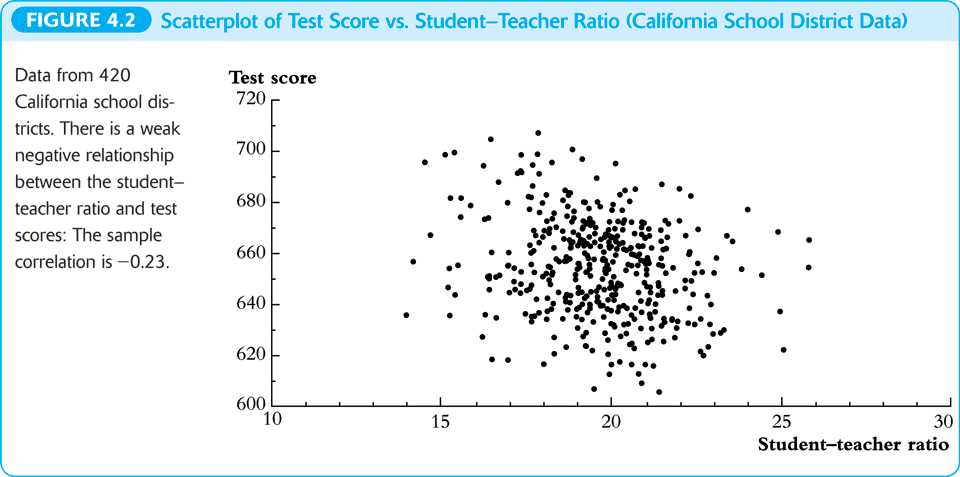
\includegraphics[width=1.0\textwidth]{img/fig-4-2.png}
\caption{\label{fig:org162f0d6}
The scatterplot between student-teacher ratios and test scores}
\end{figure}

\subsubsection*{Regression analysis}
\label{sec:orgbca3784}
After exploratory analysis, we can estimate the linear model. Although
the formula of computing \(\beta_{\text{1}}\) and \(\beta_{\text{0}}\) (Equations
\ref{eq:betahat-1} and \ref{eq:betahat-0}) seems complicated, the
practical estimation procedure is simplified by using computer software,
like R, Stata, and Eviews, which mostly involving just one-line
command or just a few clicking of the mouse. We'll see how R estimates
a linear regression model shortly. For now, let's simply present the
estimation results in the following equation,

\begin{equation}
\label{eq:testscr-str-1e}
\widehat{TestScore} = 698.93 - 2.28 \times STR
\end{equation}

We can draw the sample regression line represented by Equation
\ref{eq:testscr-str-1e} in the scatterplot to eyeball how well the
regression model fits the data.

\begin{figure}[htbp]
\centering
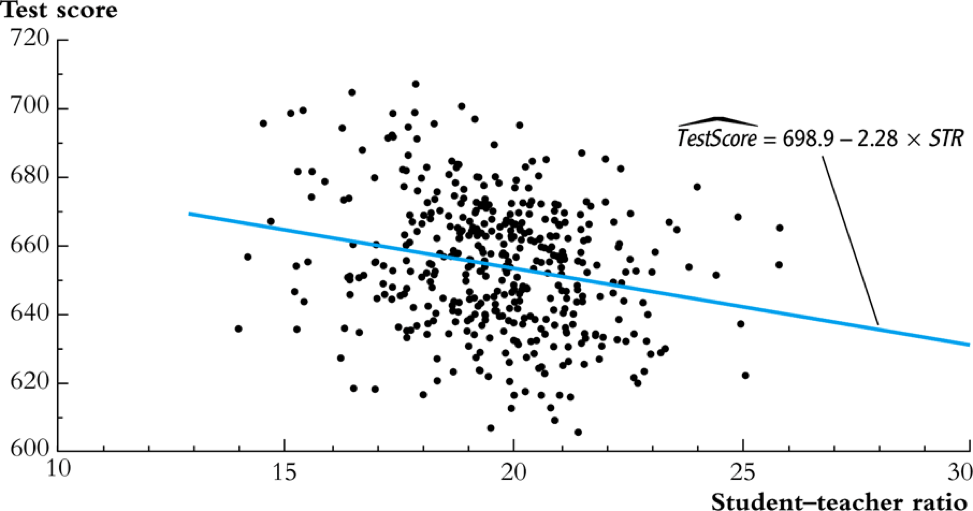
\includegraphics[width=0.85\textwidth]{img/fig-4-3.png}
\caption{The estimated regression line for the California data}
\end{figure}

\subsubsection*{Interpretation of the estimated coefficients}
\label{sec:org1843a1a}

Obtaining the estimates of the coefficients in the regression model is
not the end of a regression analysis. What need to do next includes
hypothesis tests, model specification tests, robustness (or
sensitivity) test, and interpretation. Let's first see how to
correctly interpret the estimation results.

\begin{itemize}
\item What interests us the most is the slope that tell us how much a
unit change in student-teacher ratios will cause test scores to
change. The slope of -2.28 means that an increase in the
student-teacher ratio by one student per class is, on average,
associated with a decline in district-wide test scores by 2.28 points
on the test.
\item The intercept literally means that if the student-teacher ratio is
zero, the average district-wide test scores will be 698.9. However,
it is nonsense for having some positive test scores when the
student-teacher ratio is zero. Therefore, the intercept term in this
case merely serves as determining the level of the sample regression
line.
\item The mere number of -2.28 really does not make much sense for the
readers of your research. We have to put it into the context of
California school district to avoid ridiculous results even though
the estimation itself is correct. (Read the discussion in the
paragraphs in Page 117.)
\end{itemize}


\section{Algebraic Properties of the OLS Estimator}
\label{sec:orgfb0fa9f}
\subsection{TSS, ESS, and SSR}
\label{sec:org1e11963}
\begin{itemize}
\item From \(Y_i = \hat{Y}_i + \hat{u}_i\), we can define
\begin{itemize}
\item \textbf{the total sum of squares}: \(TSS = \sum_{i=1}^n (Y_i - \bar{Y})^2\)
\item \textbf{the explained sum of squares}: \(ESS = \sum_{i=1}^n (\hat{Y}_i - \bar{Y})^2\)
\item \textbf{the sum of squared residuals}: \(SSR = \sum_{i=1}^n \hat{u}_i^2\)
\end{itemize}
\end{itemize}

Note that TSS, ESS, and SSR all take the form of "deviation from
the mean". This form is only valid when an intercept is included in the
regression model.\footnote{We are not going to prove this because it
involves higher level knowledge of linear algebra. You can estimate a
linear regression model of \(Y_i = \beta_1 X_i + u_i\), for which TSS is
simply \(\sum_i^n Y_i^2\) and ESS is \(\sum_i^n \hat{Y}_i^2\). Also, for
this model, \(\sum_i^n \hat{u}_i \neq 0\).}

\subsection{Some algebraic properties among \(\hat{u}_i\), \(\hat{Y}_i\), \(Y_i\), and \(X_i\)}
\label{sec:org7a572a0}

The OLS residuals and the predicted values satisfy the following
equations:\footnote{Equation \ref{eq:algebra-ols-1} holds only for a
linear regression model with an intercept, but Equation
\ref{eq:algebra-ols-3} holds regardless of the presence of an intercept.}
\begin{gather}
\sum_{i=1}^n \hat{u}_i = 0 \label{eq:algebra-ols-1} \\
\frac{1}{n} \sum_{i=1}^n \hat{Y}_i = \bar{Y} \label{eq:algebra-ols-2} \\
\sum_{i=1}^n \hat{u}_i X_i = 0 \label{eq:algebra-ols-3} \\
TSS = ESS + SSR \label{eq:tss-ess}
\end{gather}

\subsection{The proof of these properties}
\label{sec:org6552fbc}

Here, I just prove Equation \ref{eq:tss-ess}. The proofs for the other
equations above are in Appendix 4.3 in the textbook.

\begin{proof}

(a) Prove Equation \ref{eq:algebra-ols-1}. From Equation \ref{eq:betahat-0} we can write the OLS residuals as
$\hat{u}_i = Y_i - \hat{\beta}_0 - \hat{\beta}_1 X_i = (Y_i - \bar{Y}) - \hat{\beta}_1 (X_i - \bar{X})$. Thus
\begin{equation*}
\sum_{i=1}^n \hat{u}_i = \sum_{i=1}^n (Y_i - \bar{Y}) - \hat{\beta}_1 \sum_{i=1}^n (X_i - \bar{X})
\end{equation*}

By definition of the sample average, we have $\sum_{i=1}^n (Y_i - \bar{Y})=0$ and $\sum_{i=1}^n (X_i - \bar{X})=0$.
It follows that $\sum_{i=1}^n \hat{u}_i = 0$.

(b) To verify Equation \ref{eq:algebra-ols-2}, note that $Y_i = \hat{Y}_i + \hat{u}_i$, so
$\sum_{i=1}^n Y_i = \sum_{i=1}^n \hat{Y}_i + \sum_{i=1}^n \hat{u}_i = \sum_{i=1}^n \hat{Y}_i$. It follows that
$(1/n)\sum_{i=1}^n \hat{Y}_i = \bar{Y}$.

(c) To verify Equation \ref{eq:algebra-ols-3}, note that $\sum_{i=1}^n \hat{u}_i = 0$ implies that
$\sum_{i=1}^n \hat{u}_i X_i = \sum_{i=1}^n \hat{u}_i (X_i - \bar{X}) = \sum_{i=1}^n \left[ (Y_i - \bar{Y}) - \hat{\beta}_1 (X_i - \bar{X}) \right] (X_i - \bar{X})
= \sum_{i=1}^n (X_i - \bar{X})(Y_i - \bar{Y}) - \hat{\beta}_1 \sum_{i=1}^n (X_i -\bar{X})^2 = 0$

(d) Prove $TSS = ESS + SSR$.

\begin{equation*}
\begin{split}
TSS &= \sum_{i=1}^n (Y_i - \bar{Y})^2 = \sum_{i=1}^n (Y_i - \hat{Y}_i + \hat{Y}_i - \bar{Y})^2 \\
&= \sum_{i=1}^n (Y_i - \hat{Y}_i)^2 + \sum_{i=1}^n (\hat{Y}_i - \bar{Y})^2 + 2\sum_{i=1}^n (Y_i - \hat{Y}_i)(\hat{Y}_i - \bar{Y}) \\
&= SSR + ESS + 2\sum_{i=1}^n \hat{u}_i \hat{Y}_i \\
&= SSR + ESS + 2\sum_{i=1}^n \hat{u}_i(\hat{\beta}_0 + \hat{\beta}_1 X_i) \\
&= SSR + ESS + 2(\hat{\beta}_0 \sum_{i=1}^n \hat{u}_i + \hat{\beta}_1\sum_{i=1}^n \hat{u}_i X_i) \\
&= SSR + ESS
\end{split}
\end{equation*}
where the final equality follows from Equations \ref{eq:algebra-ols-1} and \ref{eq:algebra-ols-3}.
\end{proof}


\section{Measures of Fit}
\label{sec:org5e5049c}
\subsection{Goodness of Fit: R\(^{\text{2}}\)}
\label{sec:org74eb97a}

R\(^{\text{2}}\) is one of the commonly used measures of how well the OLS
regression line fits the data. R\(^{\text{2}}\) is the fraction of the sample
variance of Y\(_{\text{i}}\) explained by X\(_{\text{i}}\). The sample variance can be
represented with \(TSS\) and the part of sample variance explained by X
can be represented by \(ESS\). Therefore, mathematically, we can define
R\(^{\text{2}}\) as

\begin{equation}
\label{eq:rsquared}
R^2 = \frac{ESS}{TSS} = 1 - \frac{SSR}{TSS}
\end{equation}

\subsubsection*{Properties of R\(^{\text{2}}\)}
\label{sec:org250d906}

(1) \(R^2 \in [0, 1]\)

\(R^2 = 0\) when \(\hat{\beta}_1 = 0\), that is, \(X\) cannot explain the
variance in \(Y\).
\begin{equation*}
\hat{\beta}_1 = 0 \Rightarrow Y_i = \hat{\beta}_0 + \hat{u}_i
\Rightarrow \hat{Y}_i = \bar{Y} = \hat{\beta}_0 \Rightarrow ESS
= \sum_i^n (\hat{Y}_i - \bar{Y})^2 = 0 \Rightarrow R^2 = 0
\end{equation*}
\(R^2 = 1\) when \(\hat{u}_i = 0\) for all \(i = 1, \ldots, n\), that is,
the regression line fits all the sample data perfectly.
\[ \hat{u}_i = 0 \Rightarrow ESS = \sum_i^n \hat{u}_i^2 = 0
  \Rightarrow R^2 = 1 \]

(2) \(R^2 = r^2_{XY}\)

\(r_{XY}\) is the sample correlation coefficient, that is,
\[ r_{XY} = \frac{S_{XY}}{S_X S_Y} = \frac{\sum_i^n(X_i -
  \bar{X})(Y_i - \bar{Y})}{(\sum_i^n (X_i - \bar{X})^2 \sum_i^n (Y_i -
  \bar{Y})^2)^{1/2}} \]

\emph{Note}: This property holds only for the linear regression model
with a regressor and an \textbf{intercept}.

\subsubsection*{The use of R\(^{\text{2}}\)}
\label{sec:orgd1ce4c0}
\begin{itemize}
\item R\(^{\text{2}}\) is usually the first statistics that we look at for judging
how well the regression model fits the data.
\item Most computer programs for econometrics and statistics report R\(^{\text{2}}\)
in their estimation results.
\item However, we cannot merely rely on R\(^{\text{2}}\) for judge whether the
regression model is "good" or "bad". For that, we have to use some
statistics that will be taught soon.
\end{itemize}

\subsection{The standard error of regression (SER) as a measure of fit}
\label{sec:orgca2a010}

Like R\(^{\text{2}}\), the standard error of regression (SER) is another measure
of fit for the OLS regression.

\begin{equation}
\label{eq:ser}
\mathrm{SER} = \sqrt{\frac{1}{n-2}\sum^n_{i=1} \hat{u}_i^2} = s
\end{equation}

\begin{itemize}
\item SER has the units of u, which are the units of Y.
\item SER measures the average “size” of the OLS residual (the average “mistake” made by the OLS regression line).
\item The root mean squared error (RMSE) is closely related to the SER:
\[ \mathrm{RMSE} = \sqrt{\frac{1}{n}\sum^n_{i=2} \hat{u}_i^2} \]
As \(n \rightarrow \infty\), SER = RMSE.
\end{itemize}

\subsection{R\(^{\text{2}}\) and SER for the application of test scores v.s. class sizes}
\label{sec:org14b315d}
\begin{itemize}
\item In the application of test scores v.s. class sizes, R\(^{\text{2}}\) is 0.051
or 5.1\%, which implies that the regressor \emph{STR} explains only 5.1\%
of the variance of the dependent variable \emph{TestScore}.
\item SER is 18.6, which means that standard deviation of the regression
residuals is 18.6 points on the test. The magnitude of SER is so
large that, in another way, shows that the simple linear regression
model does not fit the data well.
\end{itemize}


\section{The Least Squares Assumptions}
\label{sec:orgaaa6c47}
\subsection{Assumption 1: The conditional mean of \(u_i\) given \(X_i\) is zero}
\label{sec:org98b60fd}

\begin{equation}
\label{eq:Eu}
E(u_i | X_i) = 0
\end{equation}

If Equation \ref{eq:Eu} is satisfied, then \(X_i\) is called
\textbf{exogenous}. This assumption can be a little stronger as \(E(u|X=x) = 0\)
for any value \(x\), that is \(E(u_i | X_1, \ldots, X_n) = 0\).

Since \(E(u|X=x)=0\), it follows that \(E(u)=E(E(u|X))=E(0)=0\). The
unconditional mean of \(u\) is also zero.

\begin{itemize}
\item A benchmark for thinking about this assumption is to consider an
ideal randomized controlled experiment.

Because X is assigned randomly, all other individual characteristics –
the things that make up u – are distributed independently of X, so u
and X are independent Thus, in an ideal randomized controlled
experiment, \(E(u|X = x) = 0\)

\item In actual experiments, or with observational data, we will need to
think hard about whether \(E(u|X = x) = 0\) holds
\end{itemize}

Assumption 1 can be illustrated by Figure \ref{fig:orgf2cb725}.

\begin{figure}[htbp]
\centering
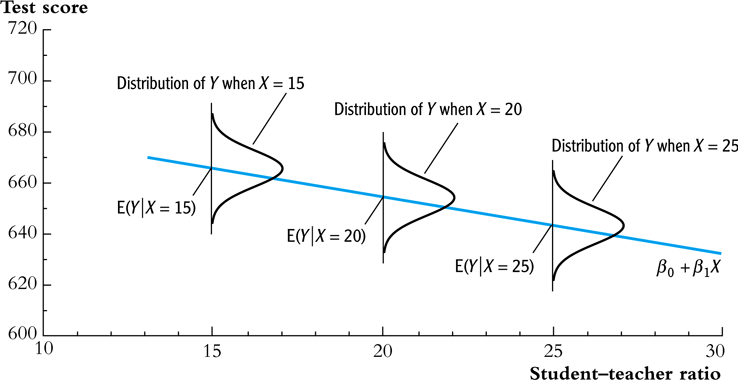
\includegraphics[width=.9\linewidth]{img/fig-4-4.png}
\caption{\label{fig:orgf2cb725}
An illustration of \(E(u|X=x)=0\)}
\end{figure}

\paragraph*{Correlation and conditional mean}
\label{sec:orgd079d67}

\[ E(u_i | X_i) = 0 \Rightarrow \cov(u_i, X_i) = 0 \]

\begin{proof}
\begin{equation*}
\begin{split}
\cov(u_i, X_i) &= E(u_i X_i) - E(u_i) E(X_i) \\
&= E(E(u_i X_i|X_i)) - E(E(u_i|X_i)) E(X_i) \\
&= E(X_i E(u_i|X_i)) - 0 \cdot E(X_i) \\
&= 0
\end{split}
\end{equation*}
where the law of iterated expectation is used twice at the second equality.
\end{proof}

It follows that \(\cov(u_i, X_i) \neq 0 \Rightarrow E(u_i|X_i) \neq 0\).

\subsection{Assumption 2: \((X_i, Y_i)\) for \(i = 1, \ldots, n\) are i.i.d.}
\label{sec:org48d038e}
\begin{itemize}
\item The individual sample \(i\), with which \((X_i, Y_i)\) is associated, is
selected randomly from the same joint distribution
\item Since \(u_i = Y_i - \beta_0 - \beta_1 X_i\), \(u_{i}\) is i.i.d.
\item The violation of the i.i.d. assumption: time series data, \(\cov(Y_t,
  Y_{t-1}) \neq 0\)
\end{itemize}

\subsection{Assumption 3: large outliers are unlikely}
\label{sec:org8f0f255}
\subsubsection*{\(0 < E(X^4_i) < \infty \text{ and } 0 < E(Y_i^4) < \infty\)}
\label{sec:orge6eb983}

\begin{itemize}
\item A large outlier is an extreme value of X or Y
\item On a technical level, if X and Y are bounded, then they have finite
fourth moments.
\item The substance of this assumption is that a large outlier can
strongly influence the results – so we need to rule out large
outliers.
\end{itemize}

\subsubsection*{The influential observations and the leverage effects}
\label{sec:org9db237b}

\begin{itemize}
\item An outlier can be detected by a scatterplot. See Figure \ref{fig:orgbef66fd}.
\end{itemize}

\begin{figure}[htbp]
\centering
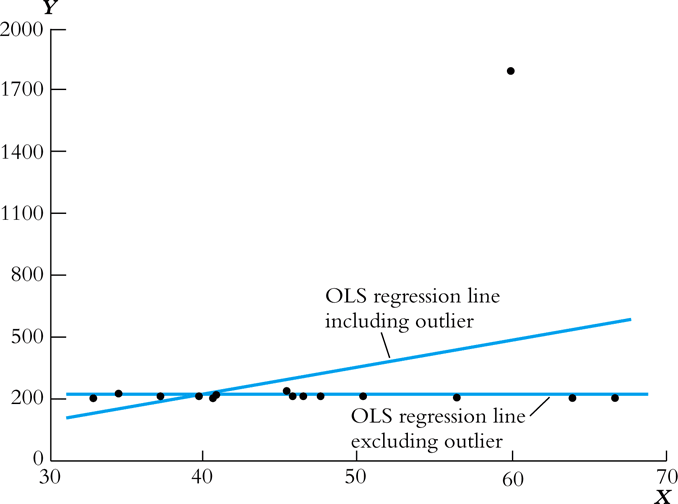
\includegraphics[width=.9\linewidth]{img/fig-4-5.png}
\caption{\label{fig:orgbef66fd}
How an outlier can influence the OLS estimates}
\end{figure}

\begin{itemize}
\item There are also formal tests for the existence of the influential
observations, some of which are coded in econometric software, like
R and Stata.
\end{itemize}



\section{Sampling Distribution of the OLS Estimators}
\label{sec:org94c3699}
\subsection{Unbiasedness and consistency}
\label{sec:org13baf04}
\subsubsection*{The unbiasedness of \(\hat{\beta}_0\) and \(\hat{\beta}_1\)}
\label{sec:orgec25f8e}
\begin{itemize}
\item The randomness of \(\hat{\beta}_0\) and \(\hat{\beta}_1\)

Since \((X_i, Y_i)\) for \(i = 1, \ldots, n\) are randomly drawn from a
population, different draws can render different estimates, giving
rise to the randomness of \(\hat{\beta}_0\) and \(\hat{\beta}_1\).

\item The unbiasedness of \(\hat{\beta}_0\) and \(\hat{\beta}_1\)

Let the true values of the intercept and the slope be \(\beta_0\) and \(\beta_1\). Based on the least squares assumption \#1: \(E(u_i|X_i) = 0\)
\[ E(\hat{\beta}_0) = \beta_0 \text{ and } E(\hat{\beta}_1) =
  \beta_1 \]

\item Show that \(\hat{\beta}_1\) is unbiased

Let's rewrite the formula of \(\hat{\beta}_1\) here
\begin{equation}
\label{eq:betahat-1a}
\hat{\beta}_1  = \frac{\sum_{i=1}^n (X_i - \bar{X})(Y_i - \bar{Y})}{\sum_{i=1}^n (X_i - \bar{X})^2}
\end{equation}

\begin{proof}
We first represent $\hat{\beta_1}$ with $\beta_1, X_i, \text{ and } u_i$

Because $Y_i = \beta_0 + \beta_1 X_i + u_i$, $Y_i - \bar{Y} =
\beta_1 (X_i - \bar{X}) + u_i - \bar{u}$, which is then plugged in
the numerator in Equation (\ref{eq:betahat-1a}). Then,
\begin{equation*}
\begin{split}
\sum_i (X_i - \bar{X})(Y_i - \bar{Y}) &= \sum_i (X_i - \bar{X})\left[\beta_1(X_i - \bar{X}) + (u_i - \bar{u}) \right] \\
&= \beta_1 \sum_i(X_i - \bar{X})^2 + \sum_i (X_i - \bar{X})u_i - \bar{u}\sum_i (X_i - \bar{X}) \\
&= \beta_1 \sum_i(X_i - \bar{X})^2 + \sum_i (X_i - \bar{X})u_i
\end{split}
\end{equation*}

Substituting this expression in Equation (\ref{eq:betahat-1a}) yields

\begin{equation}
\label{eq:betahat-1b}
\hat{\beta}_1 = \beta_1 + \frac{\frac{1}{n}\sum_i (X_i - \bar{X})u_i}{\frac{1}{n}\sum_i (X_i - \bar{X})^2}
\end{equation}

We prove that $\hat{\beta}_1$ is conditionally unbiased, from which
the unconditional unbiasedness follows naturally.
\begin{equation*}
\begin{split}
E(\hat{\beta}_1 | X_1, \ldots, X_n) &= \beta_1 + E\left\lbrace \left[\frac{\frac{1}{n}\sum_i (X_i - \bar{X})u_i}{\frac{1}{n}\sum_i (X_i - \bar{X})^2} \right] | X_1, \ldots, X_n \right\rbrace \\
&= \beta_1 + \frac{\frac{1}{n}\sum_i (X_i - \bar{X})E(u_i|X_1, \ldots, X_n)}{\frac{1}{n}\sum_i (X_i - \bar{X})^2} \\
&= \beta_1\: \text{ (by assumption 1)}
\end{split}
\end{equation*}

It follows that \[E(\hat{\beta}_1) = E(E(\hat{\beta}_1 | X_1, \ldots, X_n)) = \beta_1\]

Therefore, $\hat{\beta}_1$ is an unbiased estimator of $\beta_1$.
\end{proof}

The proof of unbiasedness of \(\hat{\beta}_0\) is left for exercise.
\end{itemize}

\subsubsection*{The consistency of \(\hat{\beta}_0\) and \(\hat{\beta}_1\)}
\label{sec:org0b0793f}
\(\hat{\beta}\) is said to be a consistent estimator
of \(\beta\) if as \(n\) goes to infinity, \(\hat{\beta}\) is in probability
close to \(\beta\), which can be denoted as \(n \rightarrow \infty,
\hat{\beta} \rarrowd{p} \beta\), or simply as \(\plim_{n \rightarrow
\infty} \hat{\beta} = \beta\).

And the law of large number states that for random i.i.d. samples \(x_1,
\ldots, x_n\), if \(E(x_i) = \mu\) and \(\var(x_i) < \infty\), then
\(\plim_{n \rightarrow \infty} \frac{1}{n}\sum_i x_i = \mu\).

Then we can show that \(\plim_{n \rightarrow \infty} \hat{\beta}_1 =
\beta_1\).

\textbf{The proof is not required to understand for this course.}

\begin{proof}
From Equation (\ref{eq:betahat-1b}) we can have
\[
\plimn (\hat{\beta}_1 -\beta_1) = \plimn \frac{\frac{1}{n}\sum_i (X_i - \bar{X})u_i}{\frac{1}{n}\sum_i (X_i - \bar{X})^2}
= \frac{\plimn \frac{1}{n}\sum_i (X_i - \bar{X})u_i}{\plimn \frac{1}{n}\sum_i (X_i - \bar{X})^2}
\]
The denominator of the last equality is just a consistent estimator of the sample variance of $X_i$, that is,
$\plimn \frac{1}{n}\sum_i (X_i - \bar{X})^2 = \sigma^2_X$

Now we need to focus on $\plimn \frac{1}{n}\sum_i (X_i - \bar{X}) u_i$. To apply the law of large numbers,
we need to find the expectation of $(X_i - \bar{X})u_i$. Given that
$E(X_i u_i) = E(E(X_i u_i |X_i)) = E(X_i E(u_i |X_i)) = 0$, we have
\[ E((X_i - \bar{X})u_i) = E(X_i u_i) + \frac{1}{n} \sum_i E(X_i u_i)
= 0 + 0 = 0  \]
So the variance of $(X_i - \bar{X})u_i$ can be expressed as
\begin{equation*}
\begin{split}
\var((X_i - \bar{X})u_i) &= E((X-\bar{X})^2 u_i^2) \\
&= E(E((X - \bar{X})^2 u_i^2|X)) \\
&= E((X-\bar{X})^2 E(u_i^2|X)) \\
&= E((X-\bar{X})^2 \sigma_u^2)\; \text{ (by the extended assumption 4. See Chapter 17)} \\
&< \infty\; \text{ (by assumption 3)}
\end{split}
\end{equation*}
Since $E((X_i - \bar{X})u_i) = 0$, $\var((X_i - \bar{X})u_i) < \infty$, and $X_i, u_i$ for $i=1, \ldots, n$ are i.i.d,
by the law of large numbers, we have
\[ \plimn \frac{1}{n} \sum_i (X_i - \bar{X}) u_i = 0 \]
Therefore, $\plimn \hat{\beta}_1 = \beta_1$.
\end{proof}

Similarly, we can also prove that \(\hat{\beta}_0\) is consistent, that
is \(\plimn \hat{\beta}_0 = \beta_0\).

\subsection{The asymptotic normal distribution}
\label{sec:org95105dc}
The central limit theory states that if \(X_1, \ldots, X_n\) with the mean
\(\mu\) and the variance \(0 < \sigma^2 < \infty\). Then,
\(\frac{1}{n}\sum_i X_i \xrightarrow{\text{ \textit d }}
N(\mu, \frac{\sigma^2}{n})\).

From the proof of consistency, we have already seen that \(E((X_i -
\bar{X})u_i) = 0\), \(\var((X_i - \bar{X})u_i) <\infty\),
and \(X_i, u_i\) for \(i=1, \ldots, n\) are i.i.d. By the central limit
theory, we know that
\[\frac{1}{n}\sum_i (X_i - \bar{X})u_i \rarrowd{d} N \left(0, \frac{1}{n}\var\left((X_i - \bar{X})u_i\right) \right) \]
It follows that from Equation (\ref{eq:betahat-1b}) and the fact that
\(\plimn \frac{1}{n}\sum_i (X_i - \bar{X})^2 = \var(X_i)\),
\(\hat{\beta}_1\) is asymptotically normally distributed as
\[ \hat{\beta}_1 \rarrowd{d} N\left( \beta_1, \sigma^2_{\hat{\beta}_1}\right) \]
where
\begin{equation}
\label{eq:sigmabeta-1}
\sigma^2_{\hat{\beta}_1} = \frac{1}{n}\frac{\var\left((X_i - \bar{X})u_i\right)}{\var(X_i)^2}
\end{equation}

Similarly, we can show that \(\hat{\beta}_0 \rarrowd{d} N(\beta_0,
\sigma^2_{\hat{\beta}_0})\), where
\begin{equation}
\label{eq:sigmabeta-2}
\sigma^2_{\hat{\beta}_0} = \frac{1}{n}\frac{\var(H_i u_i)}{\left( E(H^2_i) \right)^2}, \text{ where }
H_i = 1 - \left( \frac{\mu_X}{E(X_i^2)} \right)X_i
\end{equation}

\begin{itemize}
\item As \(\var(X_i)\) increases, \(\var(\hat{\beta}_1)\) decreases.

\begin{figure}[htbp]
\centering
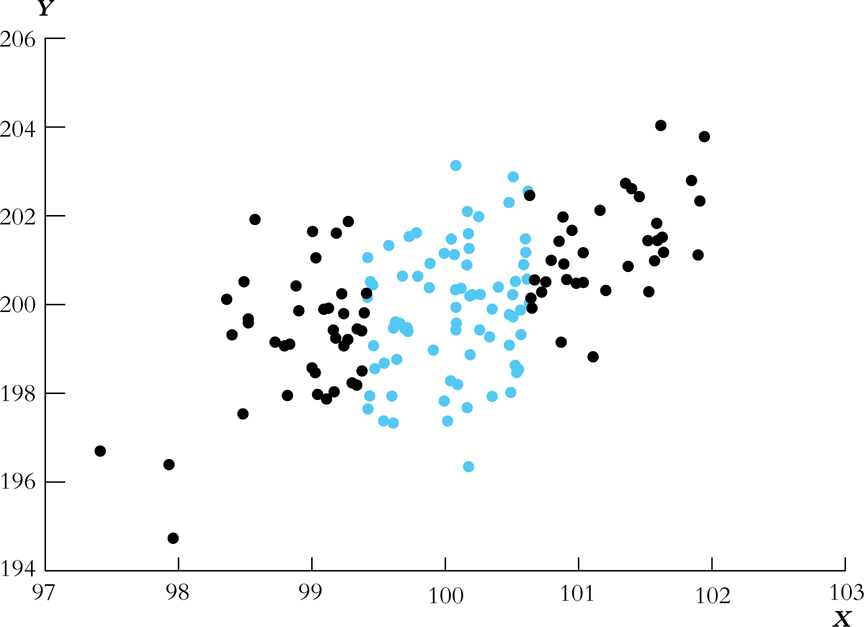
\includegraphics[width=0.85\textwidth]{img/fig-4-6.png}
\caption{\label{fig:orgc2683e1}
The Variance of \(\hat{\beta}_1\) and the variance of \(X_i\)}
\end{figure}

\item As \(\var(u_i)\) increases, \(\var(\hat{\beta}_1)\) increases.
\end{itemize}
\end{document}